\chapter{Methodology}
\label{sec:method}

\section{Formulated Research Questions}
\label{sec:rqs}

Drawing on the synthesis from \cref{sec:synthesis}, we set out four focused research questions that shape the experimental design. Each question links a concrete objective with a testable hypothesis and identifies the key methodological lever or research gap it addresses.

\begin{enumerate}
    \item \textbf{RQ1: To what extent does a transformer-based foundation model pre-trained on broad data generalize to novel robotic tasks and unseen environments?}\\[2pt]
    \textit{Objective}: Quantify zero-shot and few-shot success, failure modes and transfer gaps across varied manipulation tasks.\\[2pt]
    \textit{Hypothesis}: The model will handle moderate perceptual changes yet falter when action dynamics or task semantics shift significantly.

    \item \textbf{RQ2: Can online \ac{RL} fine-tuning restore or surpass baseline performance after large distribution shifts within tens of physical trials, and which fine-tuning strategy is most efficient?}\\[2pt]
    \textit{Objective}: Compare full-model versus partial-layer updates, on-policy versus off-policy data and safety-aware reward design. Record trials-to-recovery and asymptotic performance.\\[2pt]
    \textit{Hypothesis}: With a strong initialization from the foundation model and possibly demonstration data as a warm start, \ac{RL} adaptation will achieve substantial improvement in tens of episodes rather than thousands, representing a significant gain in sample efficiency.

    \item \textbf{RQ3: Do modular architectures that divide fast low-level control from slower high-level reasoning yield more robust real-time behavior than monolithic policies?}\\[2pt]
    \textit{Objective}: Benchmark a two-tier controller (embedded ``cerebellum'' at 200–500 Hz, cloud planner at 1–10 Hz) against an end-to-end baseline under latency, sensor noise and obstacle perturbations.\\[2pt]
    \textit{Hypothesis}: The modular design will sustain task success under latency stress whereas the monolith will degrade.

    \item \textbf{RQ4: What communication abstraction between modules best preserves global optimality while allowing independent retraining of sub-networks?}\\[2pt]
    \textit{Objective}: Evaluate interfaces such as shared latent spaces, explicit symbolic messages and probabilistic belief states in simulated pick-and-place and long-horizon assembly tasks. Measure learning stability, sample efficiency and retrain cost.\\[2pt]
    \textit{Hypothesis}: A compact stochastic latent protocol aligned with information-bottleneck theory will minimize retrain overhead while maintaining overall performance.
\end{enumerate}

This honours thesis investigates \textbf{RQ2} within the available timeframe. RQ1, RQ3 and RQ4 define the broader research landscape and motivate future work.

\section{Experimental Platform}

\subsection{Robotic Hardware}

The robotic hardware used for all real-world experiments is summarized in the tables in this section and illustrated by the STL layouts in \cref{fig:robot_parts}, the assembled SO-101 manipulators in \cref{fig:so101}, and the complete tabletop setup in \cref{fig:experimental_platform}. For real-world experiments, a physical SO-101 3D-printed robotic arm was used as the manipulator, as shown in \cref{fig:so101} \graffito{A complete material list can be found in \cref{tab:so101_bom}.}. The arm is a teleoperated tabletop platform with three rotational degrees of freedom and a parallel gripper, rigidly mounted to a flat work surface. Visual observations of the workspace were provided by fixed external RGB cameras positioned to capture both the robot and the task area. All control, data recording, and policy inference were performed on a desktop computer equipped with a consumer-grade NVIDIA RTX 3080 and RTX 5080 \acp{GPU}. Variations in the tabletop environment and object set across tasks introduced distribution shifts in object geometry and mass, surface friction, clutter, and camera viewpoint, providing a range of real-world conditions for evaluation.

\begin{figure}[ht]
    \centering
    \subfloat[Leader robot components\label{fig:leader_parts}]{
        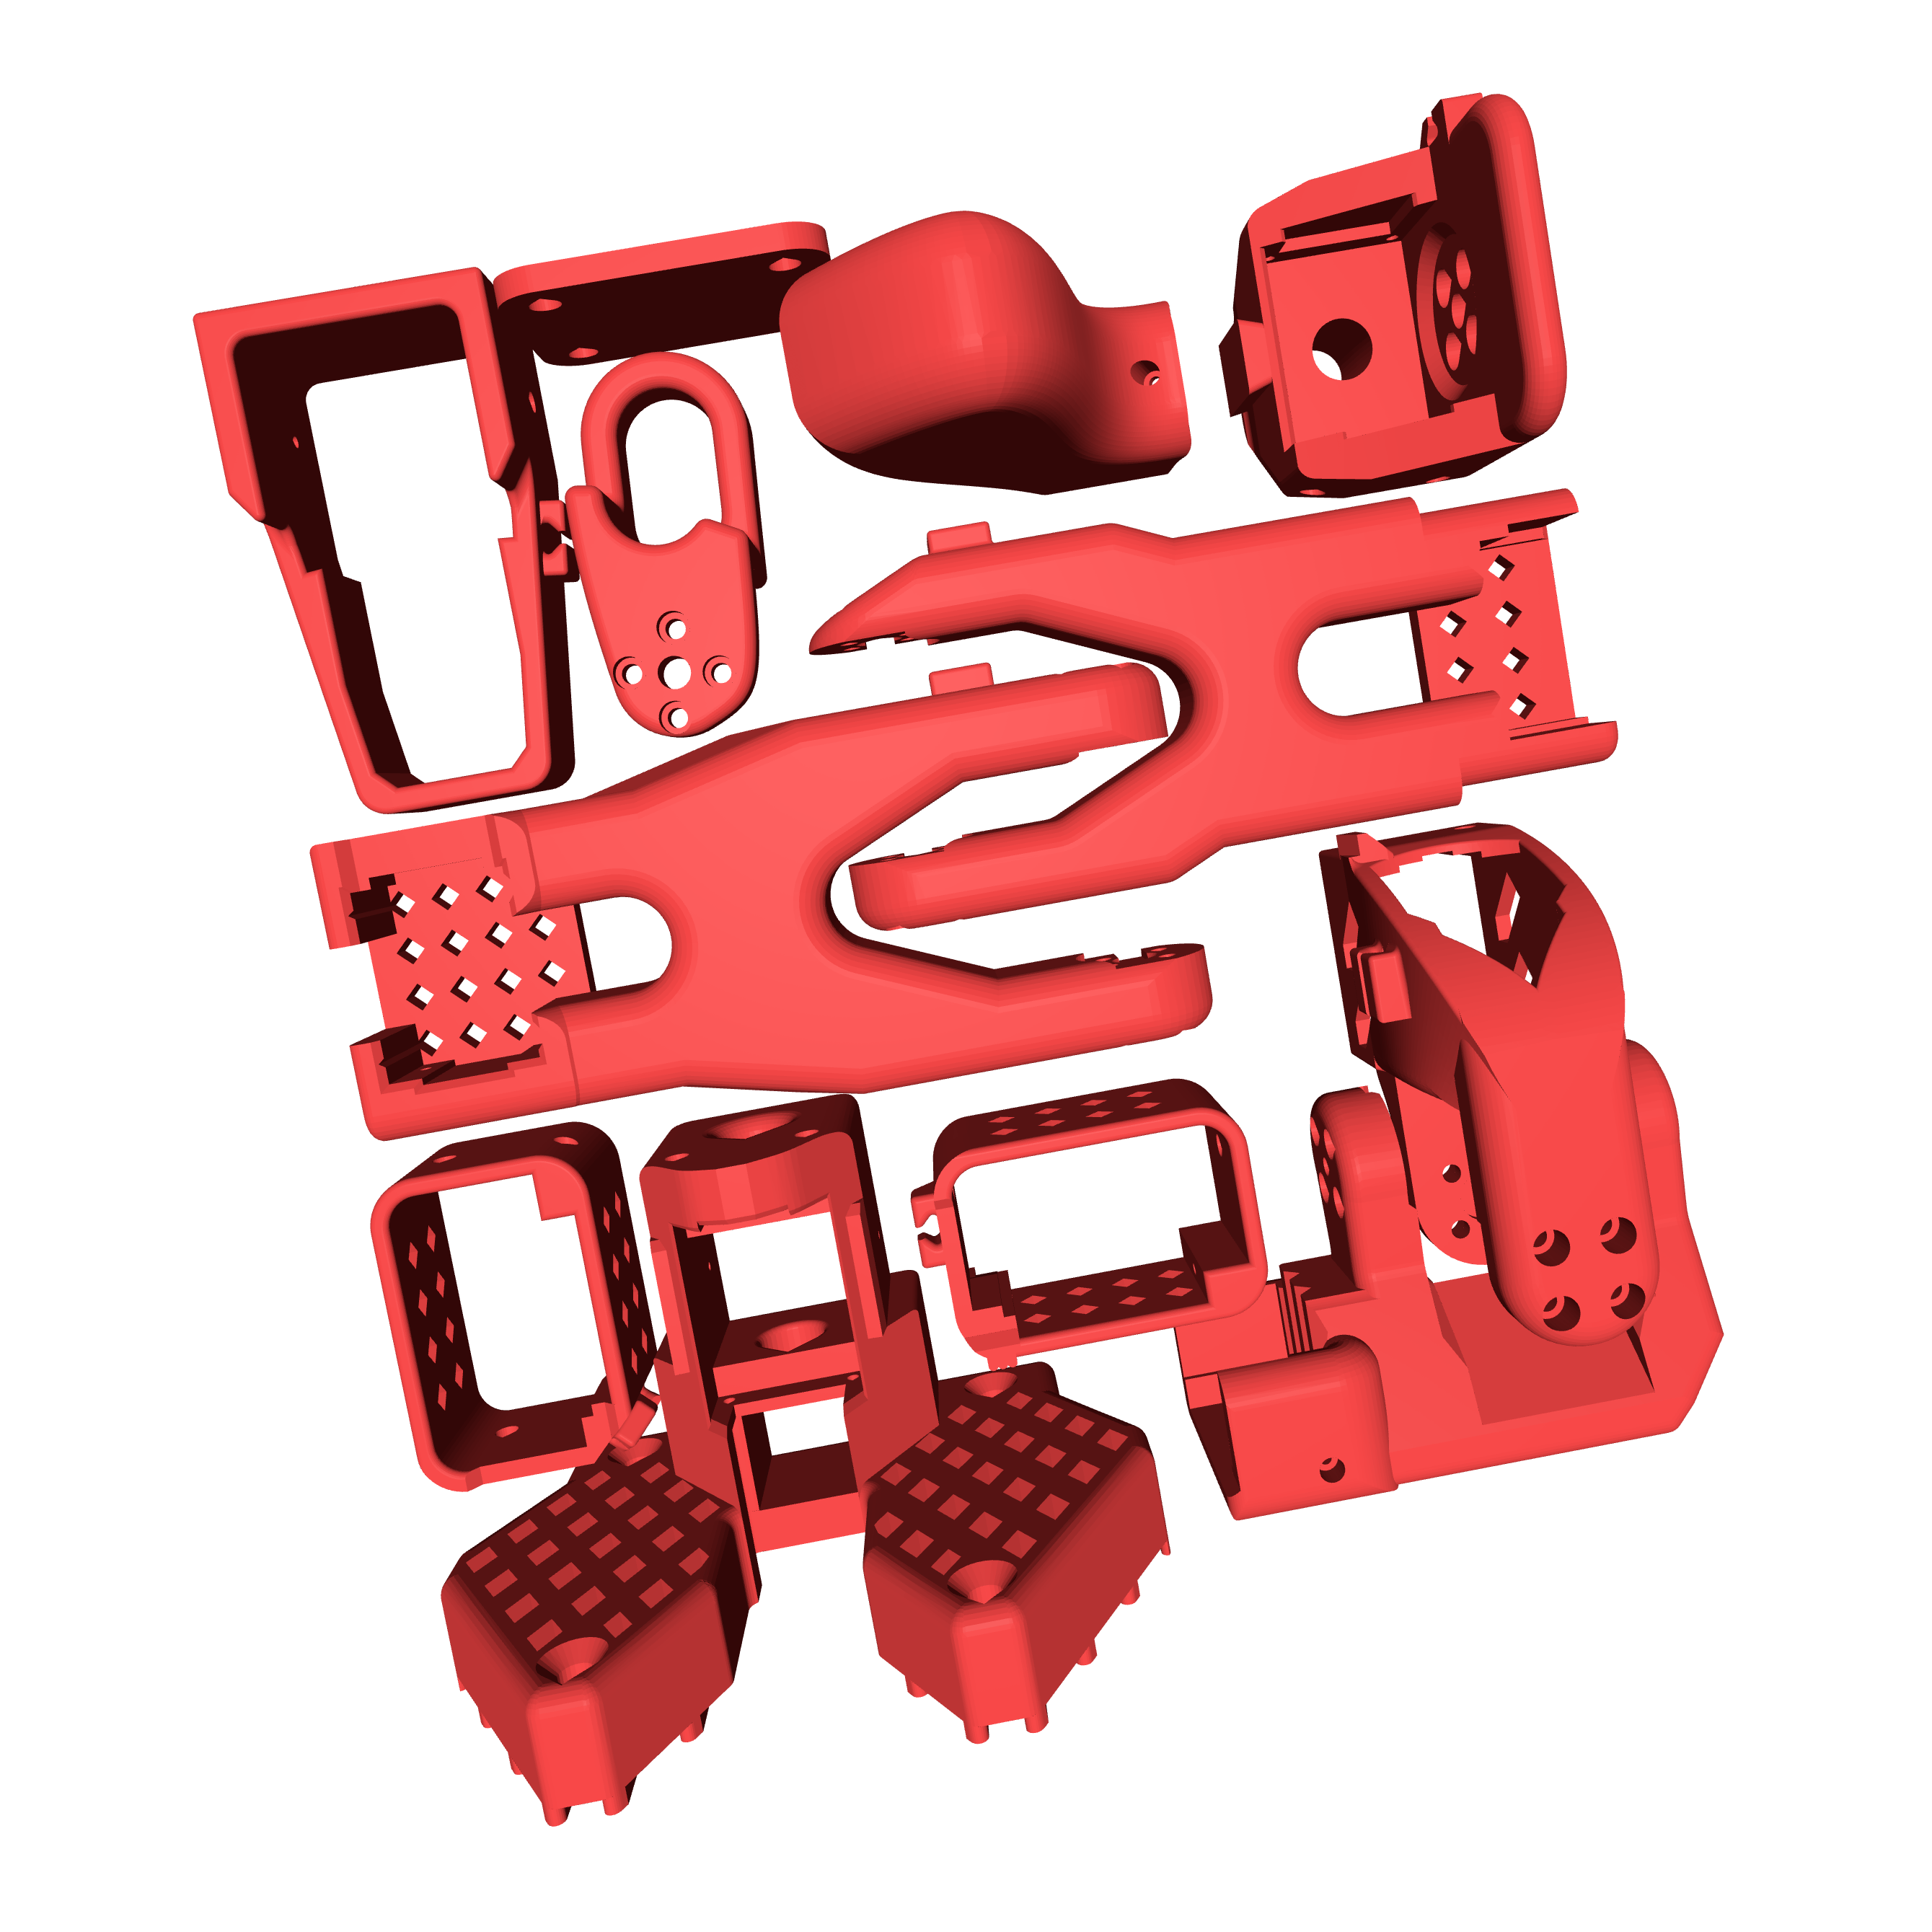
\includegraphics[width=0.45\linewidth]{Figures/leader_parts.png}
    }\hfill
    \subfloat[Follower robot components\label{fig:follower_parts}]{
        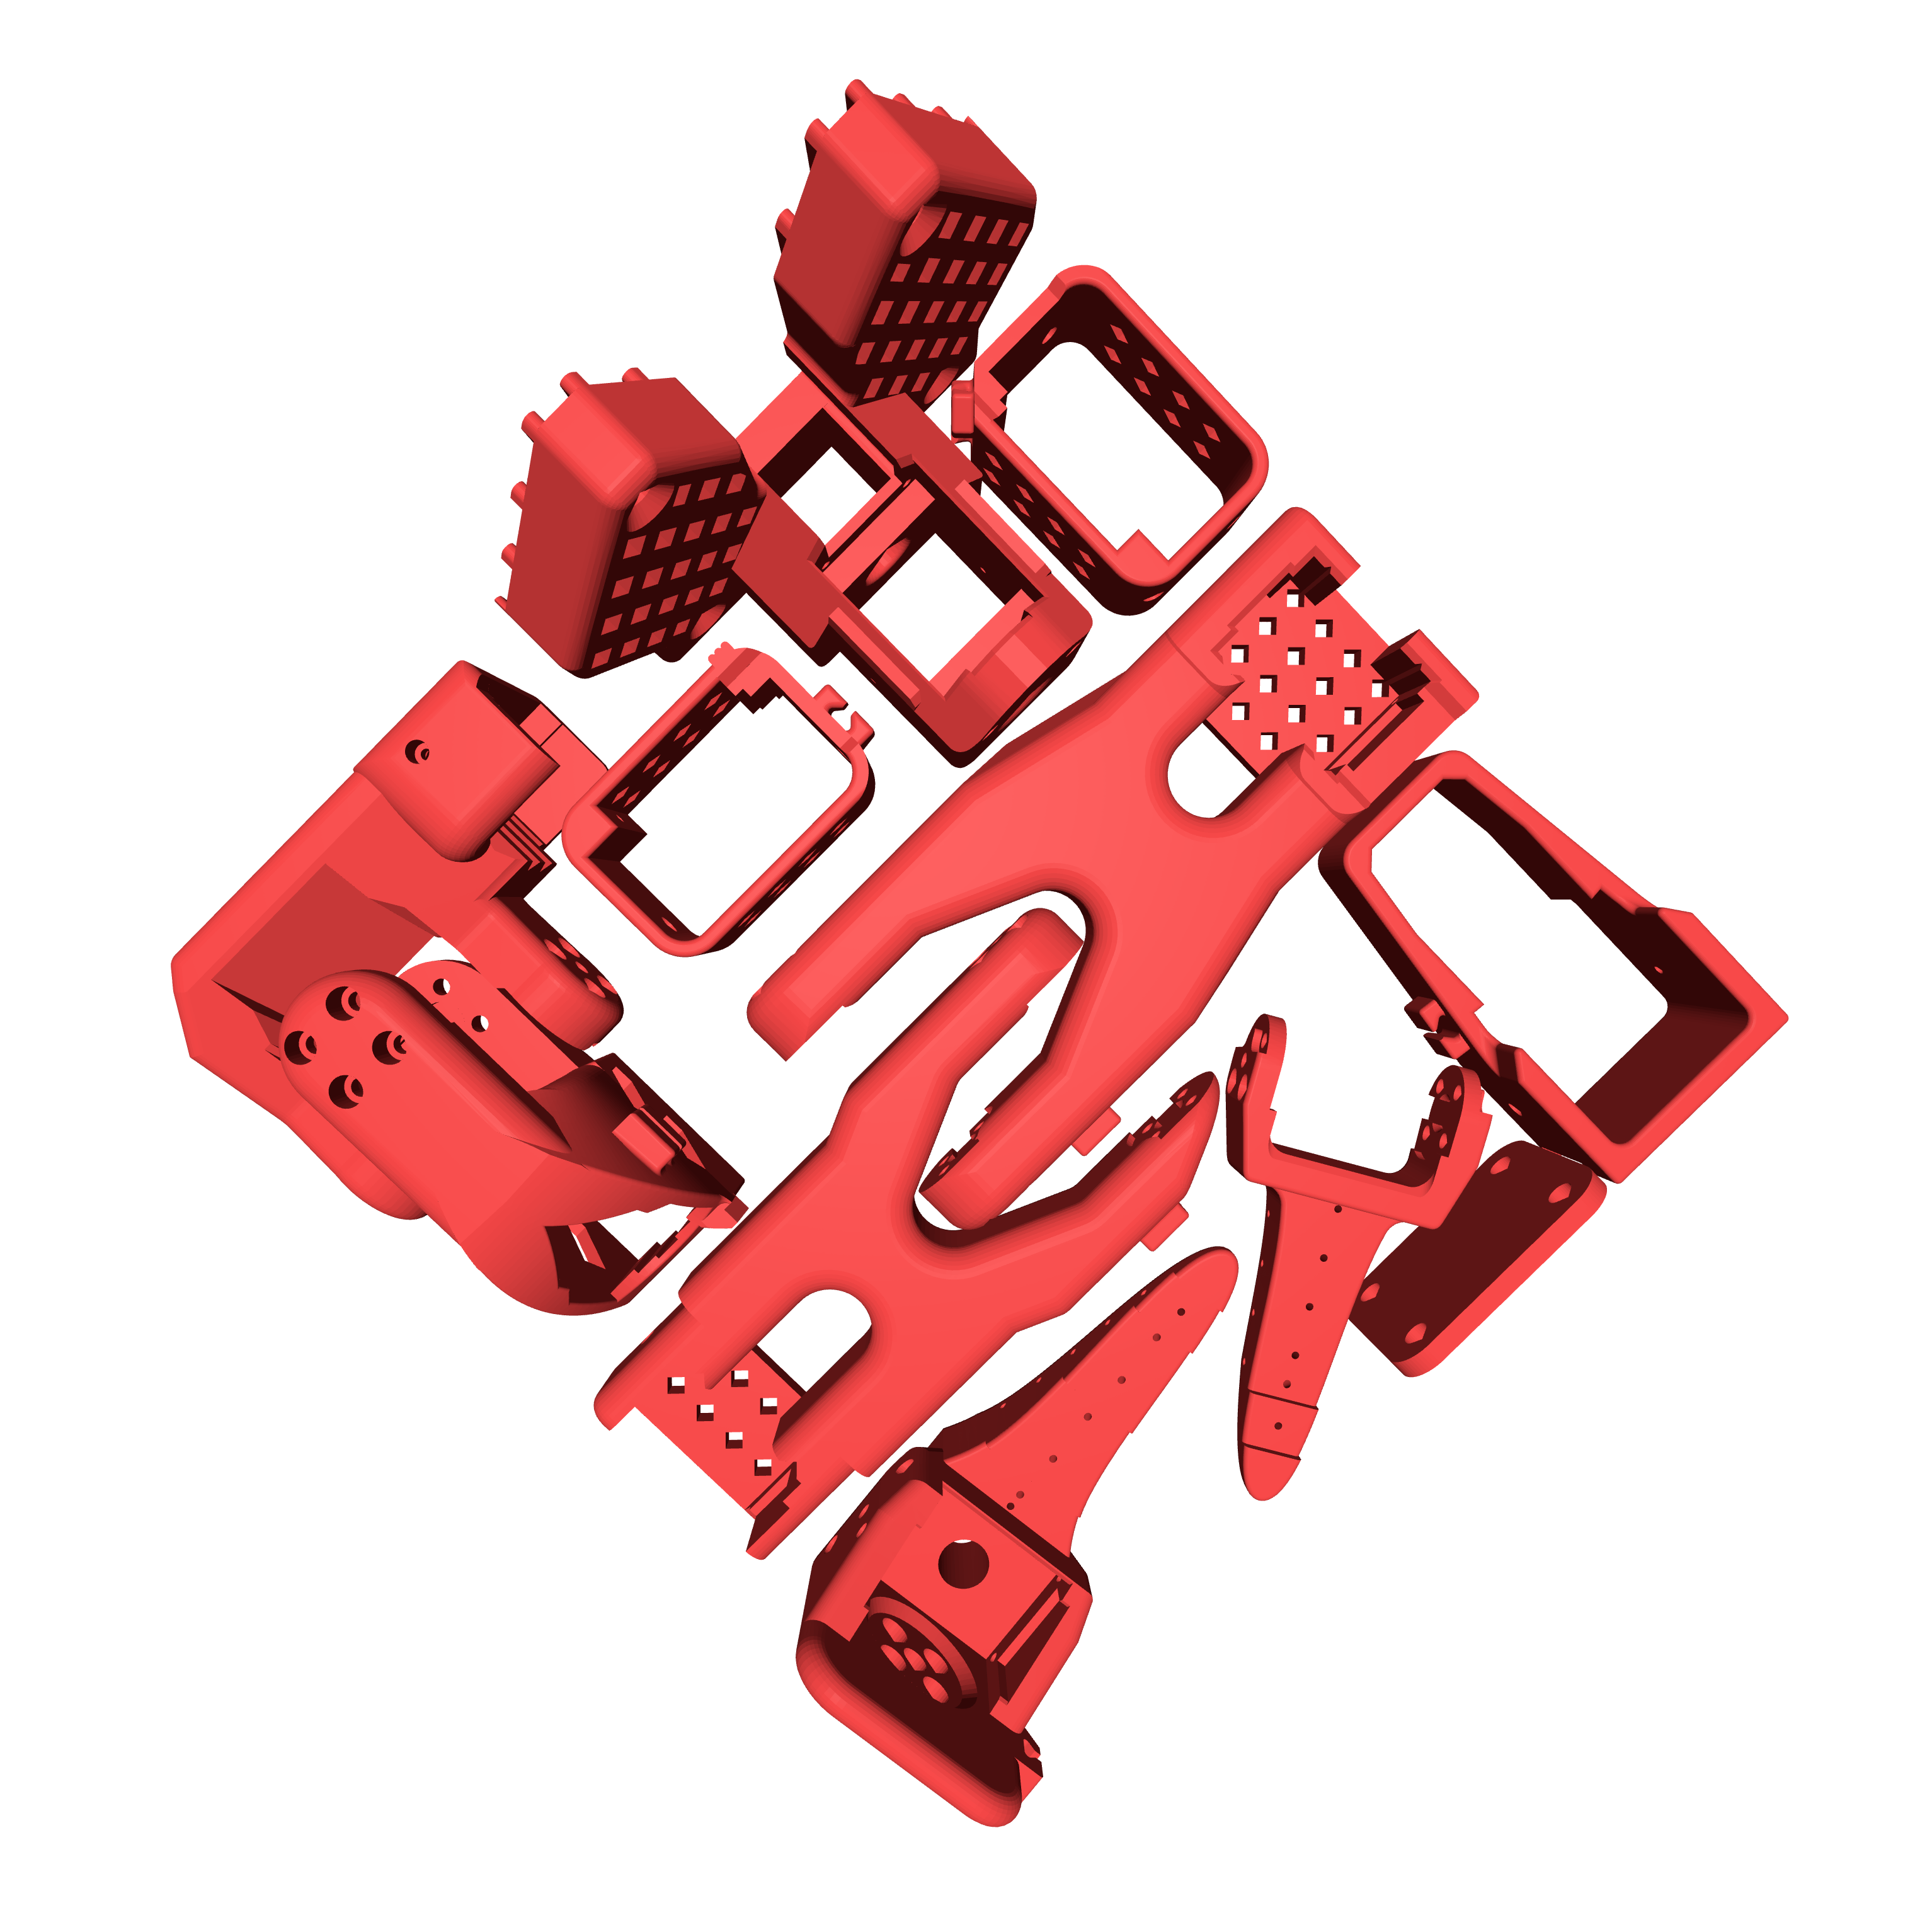
\includegraphics[width=0.45\linewidth]{Figures/follower_parts.png}
    }
    \caption{STL layouts of the leader and follower robot components arranged on the Ender 3 printer bed for fabrication.}
    \label{fig:robot_parts}
\end{figure}

\begin{figure}[ht]
    \centering
    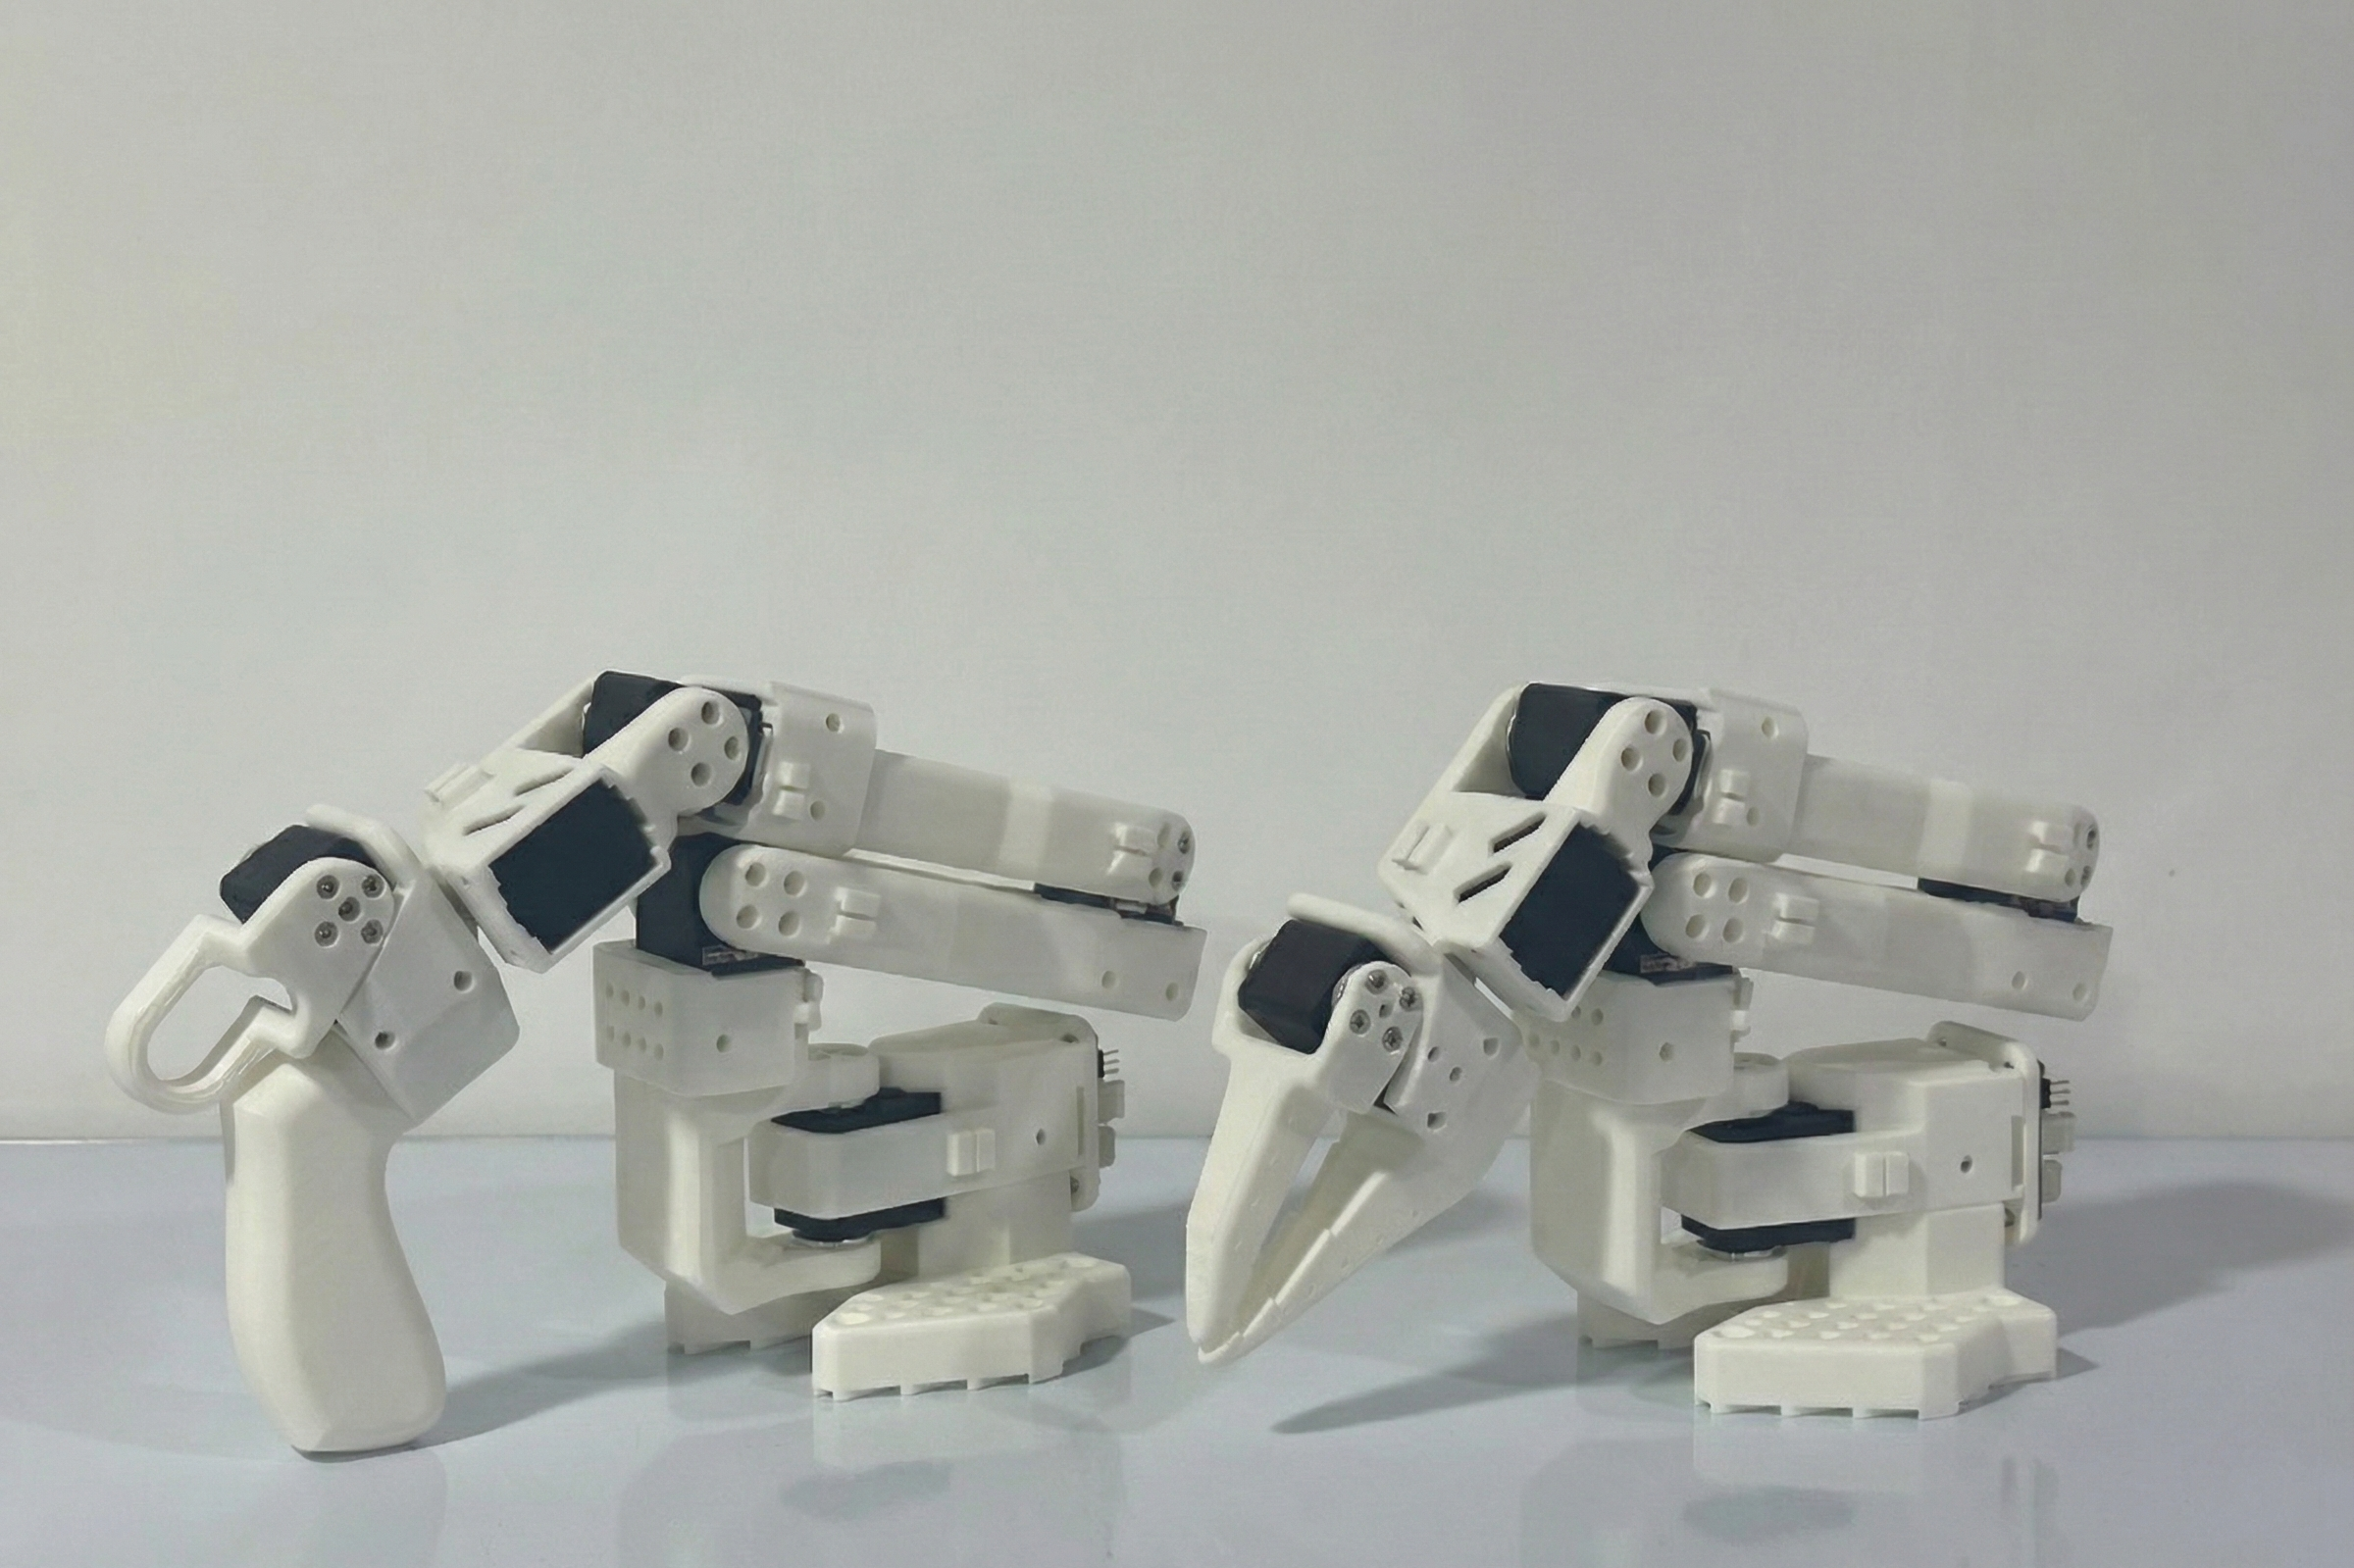
\includegraphics[width=1.0\linewidth]{Figures/so101-arms.png}
    \caption{A pair of white 3D-printed SO-101 robotic arms with black ST-3215-C0xx servos, resting side-by-side on a clean white surface.}
    \label{fig:so101}
\end{figure}

\begin{figure}[ht]
    \centering
    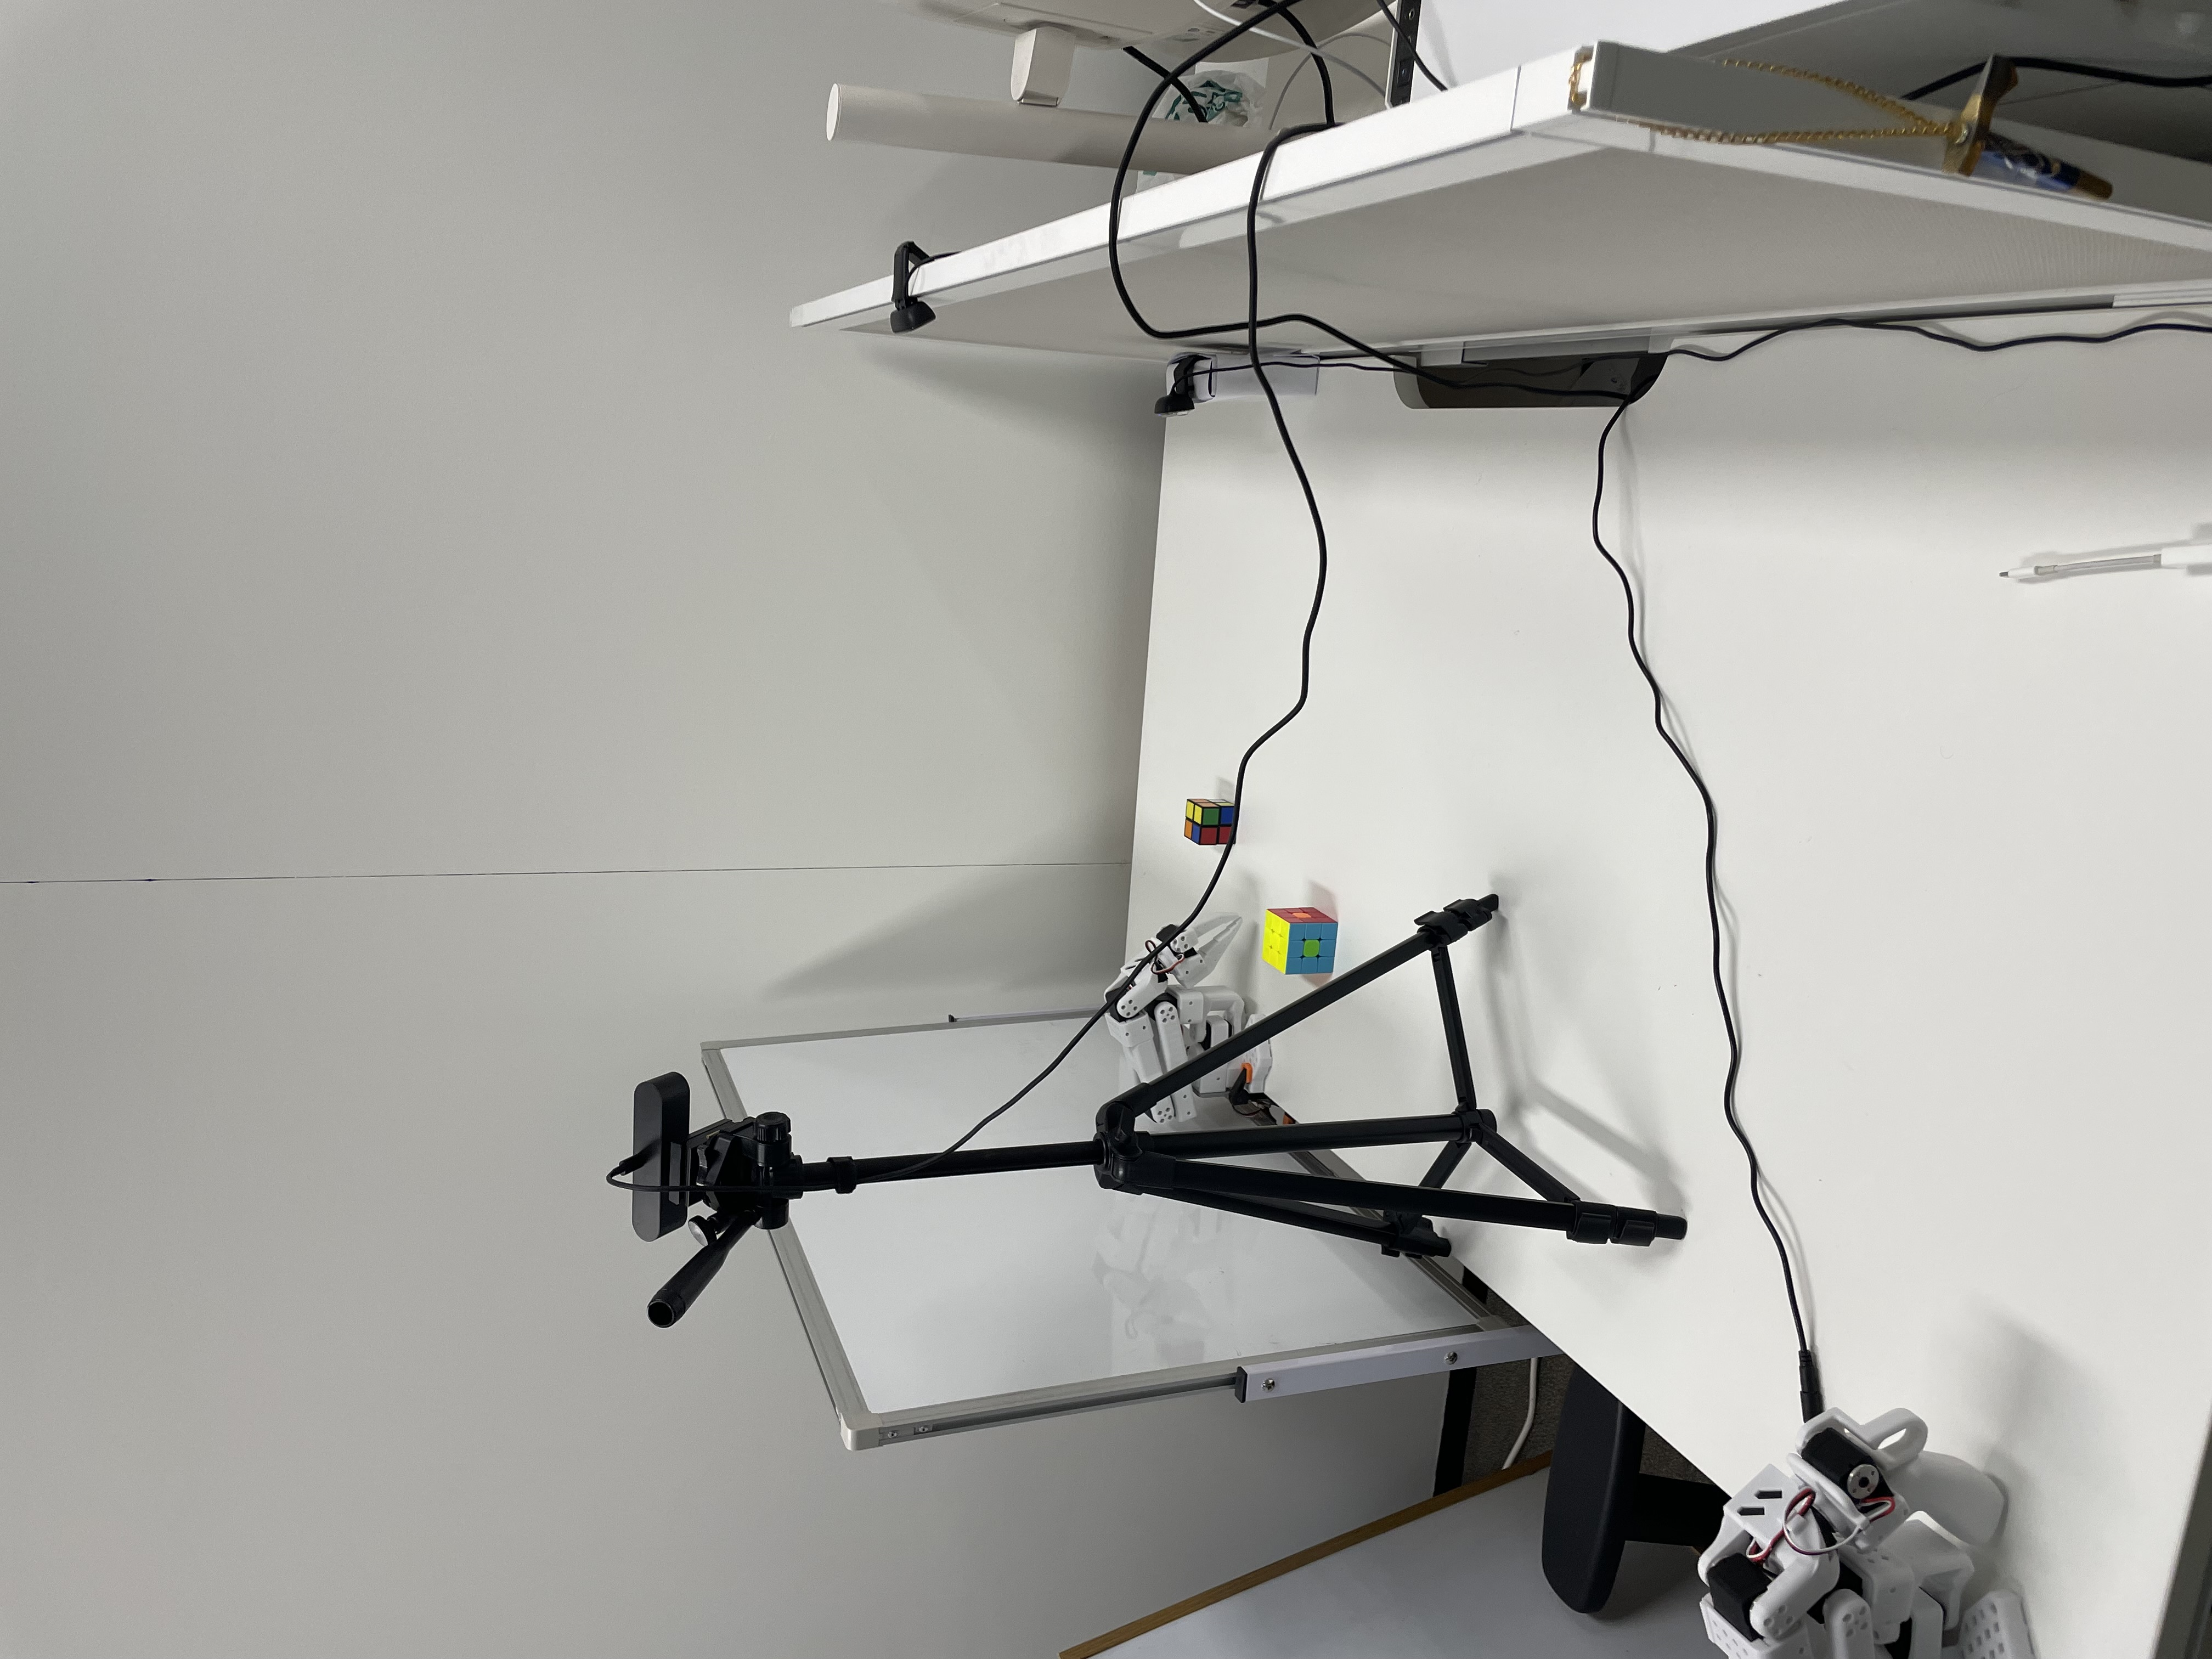
\includegraphics[width=\textwidth,angle=270]{Figures/experiment-setup.jpg}
    \caption{Experimental tabletop manipulation setup with a Lenovo top camera mounted on a tripod providing an overhead view of the white workspace, a front facing Microsoft LifeCam attached to the desk divider, and a Logitech auxiliary camera used for task monitoring, reward computation, and partitioning the workspace into discrete zones to curate balanced and diverse training data. A 3D printed SO-101 robotic arm and gripper operate on a colored training cube and a Rubik's cube on the central table, with whiteboards, an office chair, and USB cables routing connectivity between cameras and the control machine.}
    \label{fig:experimental_platform}
\end{figure}

\subsection{Sensing and Vision System}
\label{sec:method:vision_system}

The sensing and vision system was designed to provide visually simple, low-clutter observations to the visuomotor backbone and residual \ac{RL} adapters. Experiments were conducted in a predominantly white office environment with minimal background texture, including whiteboard panels placed directly behind the main manipulator to create a uniform backdrop, as visible in \cref{fig:so101,fig:experimental_platform}. This configuration reduces background clutter and high frequency visual noise, which can otherwise induce spurious correlations when policies are trained directly on pixel observations and lead to brittle behaviour under small appearance changes.

The primary camera configuration consists of a top camera mounted on a tripod that provides an overhead view of the workspace and a front facing camera attached to the desk divider, as illustrated in \cref{fig:experimental_platform}. The front camera captures lateral motions of the SO-101 arm and interactions across the horizontal extent of the task space, while the top camera supplies a bird's eye view that localises both the arm and the objects on the table with minimal occlusion. Multiple alternative camera placements were evaluated, including single front views and oblique side views\graffito{All cameras were running at the recommended 30 FPS \cite{HFHUBTUT2025}.}. These alternatives frequently suffered from occlusions when the arm or gripper passed between the camera and the objects, which degraded grasp accuracy and increased the rate of failed manipulations.

An auxiliary camera, also shown in \cref{fig:experimental_platform}, is used for task monitoring, reward computation, and partitioning the workspace into discrete zones to curate balanced and diverse training data, as illustrated in \cref{fig:partitioned_workspace}. Separating this monitoring stream from the main observation views allows the same physically fixed camera geometry to serve both control and data curation, while maintaining a consistent, noise reduced visual input for policy learning and evaluation.

\bigfigure[
    pos=ht,
    opt={width=\linewidth},
    label={fig:partitioned_workspace},
    shortcaption={Top-down view of the partitioned workspace grid.}
]{Workspace/workspace-grid.png}
{Top down view from the auxiliary monitoring camera with the workspace partitioned into a discrete grid using opencv \cite{OPENCV2000}. The zone indices are used to balance data collection across object positions and interaction regions for reward computation and dataset curation.}


\subsection{Computing Infrastructure}

All real time inference for Isaac-Gr00t and the residual \ac{RL} adapters runs on a local Linux workstation equipped with NVIDIA RTX 3080 and RTX 5080 \acp{GPU}. Initial experiments on the RTX 3080 (10\,GB VRAM) led to frequent crashes and unstable robot behaviour, as Isaac-Gr00t alone required at least 8\,GB of VRAM and left insufficient headroom for system and logging processes as displayed in \cref{tab:gpu_vram}. As a result, all final real robot experiments were executed on the RTX 5080, which provided enough memory headroom to ensure stable policy execution and reliable teleoperation. The workstation also hosted the LeRobot control stack and data logging pipeline, recording synchronized camera streams, proprioceptive states, and actions for analysis.

\begin{table}[H]
    \myfloatalign
    \scriptsize
    \begin{threeparttable}
        \caption[GPU VRAM, device counts, and cloud cost]{GPU VRAM, devices per job, and indicative cloud cost used in this work.}
        \label{tab:gpu_vram}
        
        \begin{tabular*}{\textwidth}{@{\extracolsep{\fill}} l r r r @{}}
            \toprule
            \tableheadline{GPU Model} & \tableheadline{VRAM} & \tableheadline{GPU per job} & \tableheadline{Cost per job hr (USD)} \\ 
            \midrule
            RTX~3080\tnote{a} & 10\,GB & 1 & 0.00\tnote{b} \\ 
            RTX~5080 & 16\,GB & 1 & 0.00\tnote{b} \\ 
            RTX~4090 & 24\,GB & 1 & 0.00\tnote{b} \\ 
            A100     & 40\,GB & 2 & 0.06996 \\ 
            \bottomrule
        \end{tabular*}
        
        \begin{tablenotes}
            \footnotesize
            \item[a] Isaac Gr00t requires $\ge$8\,GB of VRAM for inference. The 10\,GB capacity of the RTX~3080 operates near saturation when accounting for OS overhead and auxiliary processes.\\
            \item[b] Zero marginal cost incurred as these devices were pre-owned by the author or affiliates.
        \end{tablenotes}
    \end{threeparttable}
\end{table}

All learning of residual policies and value functions was performed remotely on Modal Cloud \cite{MODAL}. Training jobs were launched via the Modal SDK (see \cref{lst:modal}) and used two NVIDIA A100 \acp{GPU} per run, enabling efficient batched rollouts and gradient updates over the collected SO-101 trajectories. This separation of concerns placed computationally intensive training on scalable cloud hardware while reserving the local workstation for low latency control and high fidelity data capture on the physical robot.

\begin{lstlisting}[float=ht,language=Python,frame=tb,
caption={Minimal Modal SDK entrypoint that launches a two A100 cloud training run from a single \texttt{modal run train.py} command.}, label=lst:modal]
@app.function(gpu="A100:2")
def train():
  # training logic
  pass

@app.local_entrypoint()
def main():
  train.remote()
\end{lstlisting}

\subsection{Datasets and Pretraining}

Datasets are collected exclusively on the physical SO-101 3D printed arm using the HuggingFace LeRobot platform, which provides a unified interface for logging observations, actions, and task metadata. No third party robot datasets are incorporated, in order to avoid mismatches in camera geometry, sensing quality, and embodiment between this setup and external collections. For each manipulation task, a set of teleoperated demonstrations is recorded and then augmented with additional on robot rollouts generated during online learning. All trajectories share a consistent, calibrated camera configuration for the SO-101 workspace, together with proprioceptive state and low level control commands.

The visuomotor backbone is the pretrained Isaac-Gr00t policy, used in its publicly released configuration. No additional pretraining of Isaac-Gr00t is performed in this work. Learning is instead restricted to lightweight residual adapters and value functions that are trained on top of the frozen backbone using the task specific trajectories described above. Perception and instruction grounding capabilities therefore originate from Isaac-Gr00t's upstream pretraining, while the collected SO-101 dataset is used solely to specialise behaviour to the target hardware and task distribution.

\subsection{Control Architecture and Software Stack}

The control architecture is built on top of the LeRobot framework \cite{LEROBOT}, which provides a unified software stack for kinematics, low level control, and data logging for the SO-101 arm. High level components specify desired end effector poses or joint targets, while LeRobot handles conversion to hardware compatible commands and enforces joint limits and velocity constraints before streaming actions to the embedded controllers.

Geometric reasoning is implemented through a dedicated \texttt{RobotKinematics} module that wraps the \texttt{placo} library for both forward and inverse kinematics, as illustrated in \cref{lst:robot-kinematics}. The solver loads the SO-101 URDF, fixes the base, and defines a frame task at the \texttt{gripper\_frame\_link}. Forward kinematics takes joint angles in degrees, converts them to radians, updates the internal robot model, and returns a 4x4 transformation of the end effector in the world frame. This representation is used for logging, visualization, and defining Cartesian targets.

\begin{lstlisting}[float=ht,language=Python,frame=tb,
caption={Skeleton of the \texttt{RobotKinematics} helper used in the LeRobot stack. Forward and inverse kinematics run in the same URDF joint space used for control and joint limit enforcement.},
label=lst:robot-kinematics]
class RobotKinematics:
    def __init__(self, urdf_path: str,
                 target_frame_name: str = "gripper_frame_link"):
        import placo, numpy as np
        self.robot = placo.RobotWrapper(urdf_path)
        self.solver = placo.KinematicsSolver(self.robot)
        self.solver.mask_fbase(True)
        self.joint_names = list(self.robot.joint_names())
        self.tip_frame = self.solver.add_frame_task(
            target_frame_name, np.eye(4)
        )

    def forward_kinematics(self, q_deg):
        import numpy as np
        q_rad = np.deg2rad(q_deg[: len(self.joint_names)])
        for name, q in zip(self.joint_names, q_rad):
            self.robot.set_joint(name, q)
        self.robot.update_kinematics()
        return self.robot.get_T_world_frame("gripper_frame_link")

    def inverse_kinematics(self, q_deg, T_target):
        import numpy as np
        q_rad = np.deg2rad(q_deg[: len(self.joint_names)])
        for name, q in zip(self.joint_names, q_rad):
            self.robot.set_joint(name, q)
        self.tip_frame.T_world_frame = T_target
        self.solver.solve(True)
        self.robot.update_kinematics()
        q_sol = [self.robot.get_joint(n) for n in self.joint_names]
        return np.rad2deg(q_sol)
\end{lstlisting}

Inverse kinematics receives the current joint configuration and a desired 4x4 end effector pose, then uses \texttt{placo}'s \texttt{KinematicsSolver} to compute a new joint configuration. Position and orientation weights allow trading off strict pose tracking against more flexible solutions that prioritize positional accuracy over orientation when needed. The resulting joint angles are converted back to degrees, and any additional gripper joints are preserved from the input vector. In practice, this kinematics layer enables LeRobot policies and teleoperation commands that are expressed in task space to be executed as smooth joint space trajectories on the physical arm.

\subsection{Teleoperation Interface and Data Collection Pipeline}

Demonstration data are collected using LeRobot's leader follower teleoperation interface for the SO-101 arm. As shown in \cref{lst:lerobot-teleop}, a single command launches a process that configures one SO-101 as the leader device and a second SO-101 as the follower. The leader arm streams its measured joint angles over serial in real time, and the follower arm tracks these targets with low latency, reproducing the demonstrated motion in the main workspace.

During teleoperation, LeRobot records synchronized trajectories that include joint positions, gripper state, and derived end effector poses from the kinematics module, along with timestamps. When camera streams are active, RGB frames are captured and time aligned with the robot state, producing pixel based demonstrations suitable for visuomotor learning. The resulting trajectories are written in LeRobot's dataset v3 format, organized into episodes that can be directly consumed by the subsequent behavior cloning and residual reinforcement learning pipelines without additional conversion.

\begin{lstlisting}[float=ht,frame=tb,
caption={Command used to launch the SO101 leader follower teleoperation pair for data collection. The follower arm receives low latency joint targets from the leader device over serial, enabling real world demonstration recording.}, 
label=lst:lerobot-teleop]
python -m lerobot.scripts.teleoperate \
    --robot.type=so101_follower \
    --robot.port=/dev/ttyACM1 \
    --robot.id=so101_follower_arm \
    --teleop.type=so101_leader \
    --teleop.port=/dev/ttyACM0 \
    --teleop.id=so101_leader_arm
\end{lstlisting}

\subsection{Safety Protocols}

Safety constraints are implemented in the LeRobot action processing pipeline. Before any data collection or reinforcement learning, joint limits are calibrated using the built in \texttt{lerobot-find-joint-limits} utility shown in \cref{lst:joint-limits}. 

\begin{lstlisting}[float=ht,frame=tb,
caption={Command used to identify per-joint limits for the SO101 follower arm. The resulting configuration file is reused at training and deployment time to clip actions to a safe workspace.},
label=lst:joint-limits]
lerobot-find-joint-limits \
  --robot.type=so101_follower \
  --robot.port=/dev/ttyACM1 \
  --robot.id=so101_follower_arm \
  --teleop.type=so101_leader \
  --teleop.port=/dev/ttyACM0 \
  --teleop.id=so101_leader_arm \
  --config_path=src/lerobot/configs/joint_limit_config.json
\end{lstlisting}

The end effector processor in \cref{lst:ee-safety} clips Cartesian poses to a bounded workspace and limits per step translations, while joint space utilities cap relative motor targets (\texttt{max\_relative\_target}), gripper commands are clipped to a safe range, the motor bus disables torque on disconnect, and reset routines interpolate trajectories in small steps. Together, these mechanisms provide a simple safety layer around teleoperation and RL control on the SO-101 arm.

\begin{lstlisting}[float=ht,language=Python,frame=tb,
caption={End effector safety processor in the LeRobot stack. The step clips the commanded pose to a bounded workspace and limits the maximum translation between consecutive commands.},
label=lst:ee-safety]
@dataclass
class EEBoundsAndSafety(RobotActionProcessorStep):
    end_effector_bounds: dict
    max_ee_step_m: float = 0.05
    _last_pos: np.ndarray | None = field(default=None, init=False, repr=False)

    def action(self, action: RobotAction) -> RobotAction:
        # current target position in Cartesian space
        pos = action.ee_pose[:3, 3]

        # clip to workspace bounds
        pos = np.clip(
            pos,
            self.end_effector_bounds["min"],
            self.end_effector_bounds["max"],
        )

        # limit per step motion to max_ee_step_m
        if self._last_pos is not None:
            dpos = pos - self._last_pos
            n = float(np.linalg.norm(dpos))
            if n > self.max_ee_step_m and n > 0:
                scale = self.max_ee_step_m / n
                pos = self._last_pos + dpos * scale

        self._last_pos = pos
        action.ee_pose[:3, 3] = pos
        return action
\end{lstlisting}

\section{Evaluation Metrics}
\label{sec:method:evaluation_metrics}

To rigorously evaluate the generalization capabilities of the $\mResRL$ system compared to $\mBase$ and $\mRL$ baselines, this study moves beyond binary success rates to employ a fine-grained analysis of task execution. The evaluation framework centers on the \ac{DTP} metric, which quantifies partial success to isolate specific failure modes across perception, kinematics, and dynamics.

\subsection{Primary Metric: Discretized Task Progress (DTP)}
Standard binary metrics often obscure the underlying causes of failure in robotic manipulation. A failure to grasp an object (control error) is fundamentally different from a failure to locate it (perception error), yet both result in a zero-success score. To resolve this ambiguity, a continuous progress score $P_{\text{task}} \in [0, 1]$ is assigned to every trial instead of using $P_{\text{task}} \in \{0, 1\}$ \cite{PI02024}. This enables the measurement of the semantic stage reached by the policy.

As defined in \cref{tab:dtp_definitions}, each task is segmented into four semantic milestones. These scores are aggregated to calculate the \ac{MP} across $N$ trials,
\begin{equation}
MP = \frac{1}{N} \sum_{i=1}^{N} P_{\text{task}}^{(i)},
\end{equation}
where a higher $MP$ indicates robust partial completion and helps diagnose the specific bottleneck of a given policy.

\begin{table}[H]
  \myfloatalign
  \scriptsize
  \caption{Definitions of discretized task progress ($P_{\text{task}}$) milestones. This framework distinguishes between early perceptual failures and late-stage manipulation failures.}
  \label{tab:dtp_definitions}
  \begin{tabularx}{\textwidth}{c X X c}
    \toprule
    \textbf{Score} & \textbf{Semantic Stage} & \textbf{Definition} & \textbf{Testing Focus} \\
    \midrule
    0.00 & Detection Failure & The robot fails to approach the object or moves to an incorrect location. & Vision (VLA) \\
    0.25 & Approach/Contact & The end-effector makes physical contact with the target object but fails to initiate a stable grasp. & Calibration/IK \\
    0.50 & Grasp Stability & The object is successfully lifted $>5$cm off the surface but is dropped during transport. & Dynamics (RL) \\
    0.75 & Transport & The object is transported to within $5$cm of the target zone but placement fails (for example, collision). & Control (RL) \\
    1.00 & Task Success & The object is placed in the target state and the robot retreats successfully. & End-to-End \\
    \bottomrule
  \end{tabularx}
\end{table}

\subsection{Trial Protocol: The 5--5--10 Split}
\label{sec:method:trial_protocol}

For each combination of \textit{Method} ($\mBase$, $\mRL$, $\mResRL$) and \textit{Task}, the policy is evaluated with a fixed budget of $20$ real-world rollouts, indexed $i = 1,\dots,20$. Throughout, the method labels are written in small caps: $\mBase$ denotes the supervised base policy trained on offline demonstrations, $\mRL$ denotes the \ac{RL} baseline trained from scratch without access to $\mBase$, and $\mResRL$ denotes the residual \ac{RL} adapter composed with a frozen copy of the base policy. In $\mResRL$, \ac{RL} updates only the residual head; the base policy parameters are not modified.

A budget of $20$ trials balances statistical reliability with experimental feasibility. Fewer rollouts would make it difficult to distinguish systematic effects from stochastic variation, while substantially more rollouts would be prohibitive given the time required for data collection, training, and deployment across all method–task pairs. These trials follow a structured ``5--5--10'' protocol that separates calibration, kinematic reach, and generalization performance:

\begin{itemize}
    \item \textbf{Trials 1--5: \acf{ID}.}
    The target object is placed near the center of the workspace in an optimal configuration consistent with the training data distribution. This block serves as a sanity check to verify that the policy can complete the task under nominal conditions. It isolates the baseline competency of the model before introducing shifts; if persistent failure occurs in this phase, it indicates a fundamental failure in policy learning rather than a lack of robustness.
    
    \item \textbf{Trials 6--10: Dynamic Perturbation.}
    Active perturbations are applied during the rollout to stress the closed-loop reactive capabilities of the policy. These include manual non-destructive interference (e.g., nudging the object or the robot arm during trajectory execution) or initializing the robot in unstable states. This phase explicitly tests the \emph{residual} nature of the architecture, determining if the RL component can correct for deviations that would typically cause an open-loop $\mBase$ policy to fail.
    
    \item \textbf{Trials 11--20: \acf{OOD}.}
    The object is presented under added distribution conditions designed to test systematic generalization. This includes \ac{OOD} factors such as randomized poses, altered lighting conditions, added visual clutter, or changes in surface friction. These ten trials constitute the primary generalization regime, evaluating whether the policy has learned robust semantic representations and physical dynamics rather than memorizing specific visual cues.
\end{itemize}

The \ac{DTP} score $P_{\text{task}}^{(i)}$ is recorded for each trial in all three phases. Aggregate metrics are reported both over all $20$ trials and in specific subsets to isolate the gains provided by the residual RL adapter.

\subsection{Generalization and Transfer Metrics} 

To quantify the specific benefit of the RL adapter, two derived metrics are employed utilizing the DTP scores collected under \ac{OOD} conditions (randomized initialization and dynamics shifts).

\begin{itemize}
    \item \textbf{Generalization Score ($J_{\text{gen}}$):} calculated strictly on the final subset of trials within the \ac{OOD} protocol. This serves as the primary indicator of a model's robustness to unseen environments,
    \begin{equation}
        J_{\text{gen}} = \frac{1}{10} \sum_{i=11}^{20} P^{(i)}_{\text{task}}.
    \end{equation}
    \item \textbf{Transfer Gap ($\Delta_{gen}$):} measures the explicit performance gain provided by $\mResRL$ over the frozen $\mBase$. This is defined as,
    \begin{equation}
        \Delta_{gen} = J_{\text{gen}}(\mResRL) - J_{\text{gen}}(\mBase).
    \end{equation}
    A positive $\Delta_{gen}$ validates the hypothesis that online RL adaptation effectively bridges the sim-to-real or distribution gap that limits the frozen $\mBase$.
\end{itemize}

\subsection{Comprehensive Evaluation Protocol} 
Beyond progress scores, secondary metrics are tracked to ensure safety and statistical validity across all experimental phases. These are summarized in \cref{tab:comprehensive_metrics}.

{\small
\begin{longtable}{L{0.3\textwidth}L{0.62\textwidth}}
    \caption{Comprehensive evaluation metrics used in this work. The metrics of the groups quantify (i) task outcomes such as overall Task~Success~Rate, (ii) learning dynamics like Adaptation~Speed and Continual~Learning performance, (iii) safety and robustness through explicit Failure~Counts and constraint satisfaction, and (iv) statistical and qualitative diagnostics that verify the reliability and interpretability of observed gains.}
    \label{tab:comprehensive_metrics} \\
    \toprule
    \textbf{Metric} & \textbf{Description} \\
    \midrule
    \endfirsthead
    
    \multicolumn{2}{l}{\textit{(continued from previous page)}} \\
    \midrule
    \textbf{Metric} & \textbf{Description} \\
    \midrule
    \endhead
    
    \midrule \multicolumn{2}{r}{\textit{(continued on next page)}} \\
    \endfoot
    
    \bottomrule
    \endlastfoot
    
    Task Success Rate & Percentage of trials in which the robot completes the task across nominal and shifted conditions. \\
    \midrule
    Adaptation Speed & Number of episodes required to recover a target fraction of baseline performance. \\
    \midrule
    Safety and Failure Count & Number of unsafe incidents and constraint satisfaction, separated into minor and major failures. \\
    \midrule
    Continuous Control Performance & Trajectory error, task completion time, and continuous placement scores before and after adaptation. \\
    \midrule
    Continual Learning Metrics & Forward transfer and forgetting when learning sequential tasks. \\
    \midrule
    Ablation Comparisons & Performance of system variants to isolate the contribution of each module. \\
    \midrule
    Statistical Significance & Confidence intervals or hypothesis tests on success rates. \\
    \midrule
    Qualitative Evaluation & Behavioural observations such as smoothness, strategy changes, or motion quality. \\
\end{longtable}
}

% \section{Implementation Roadmap}

% \subsection{System Development Phases for RQ2}
% \label{sec:rq2_phases}

% The implementation of RQ2 is organised into four phases that structure the progression from baseline control to robustness evaluation. The phases provide a conceptual scaffold for the methodology rather than a strict chronological schedule. \cref{tab:implementation_phases} summarises the main objectives and key dependencies within each phase.

% \begin{table}[H]
%   \myfloatalign
%   \caption[System development phases for RQ2]{System development and evaluation phases for the residual \ac{RL} pipeline on a foundation-model-based visuomotor controller.}
%   \label{tab:implementation_phases}
%   \begin{tabularx}{\textwidth}{lX}
%     \toprule
%     \tableheadline{Phase} & \tableheadline{Main objectives and dependencies} \\
%     \midrule
%     Environment and controller setup &
%     Specification of the robotic platform and manipulation tasks; configuration of baseline controllers (e.g., \ac{IK} or \ac{PID}) and safety monitors for joint limits and collisions; activation of logging and task variation to support robust evaluation and later analysis. \\
%     \midrule
%     Residual \ac{RL} integration &
%     Freezing the pre-trained \ac{VLA} backbone; defining the interface between the backbone policy and the residual controller; selecting a continuous-control \ac{RL} algorithm (such as \ac{PPO}) and tuning hyperparameters on perturbed tasks to obtain stable learning behaviour and informative learning curves. \\
%     \midrule
%     Physical deployment on hardware &
%     Integration of the robotic platform with perception (\ac{RGB-D} sensing) and middleware; verification of baseline reachability and perception quality; cautious deployment of learned policies under conservative safety limits; iterative refinement of filtering and impedance settings to compensate for latency, noise, and dynamics mismatches. \\
%     \midrule
%     Robustness and ablation study &
%     Evaluation across multiple tasks and perturbations using success, adaptation, and safety metrics; comparison against ablated variants (for example, without pre-training or without safety monitors) to isolate the contribution of individual components; consolidation of results and observations into a consistent dataset for analysis and dissemination. \\
%     \bottomrule
%   \end{tabularx}
% \end{table}

\section{Risk Assessment and Mitigation}

This section presents a comprehensive risk assessment and mitigation plan for the SO-101 robotic foundation-model pipeline. It identifies six key risk categories: (i) reinforcement‐learning convergence, (ii) transformer latency and memory constraints, (iii) hardware or sensor failures, (iv) evaluation bias, (v) scope creep and time management, and (vi) module integration complexity, providing a succinct description of each threat alongside targeted countermeasures. For each of these risks, the following subsections outline the specific concern, along with corresponding mitigation strategies to ensure safe and efficient execution of the project.

\subsection{RL Convergence Issues}

Online fine-tuning may be slow, unstable, or converge to suboptimal behaviors, risking wasted real-robot trials. Mitigation strategies focus on the following: Employ off-policy or batch \ac{RL} with replay buffer; start with safe exploration (low learning rate, ensemble value functions); consider \ac{MAML} pretraining for fast adaptation; maintain human oversight for corrective demos in early trials.

\subsection{Transformer Too Slow or Memory-Heavy}
A Large multimodal model may only run at $\sim$1\,Hz or exceed onboard memory, preventing real-time control. To address this risk, the following measures are adopted: Apply knowledge distillation or model compression to create a smaller policy network; use a two-process architecture (heavy model offboard, low-level reflexes onboard); quantize weights or adopt efficient transformer variants with sparse/windowed attention.

\subsection{Unexpected Hardware Failures}
Gripper malfunctions, camera glare, or other hardware issues could disrupt experiments and cause downtime. To reduce the impact of such failures, the system is designed as follows: Add redundancy (force-sensor reflexes to detect and retry bad grasps); enable teleoperation/manual override; install secondary cameras or object markers for fallback sensing; schedule early experiments and keep spare parts on hand.

\subsection{Evaluation Bias or Insufficient Testing}
Overly easy or overly hard test conditions may misrepresent performance and generalization capabilities. To counteract this risk, the evaluation protocol incorporates the following: Leverage established benchmarks and a spectrum of shifts (mild to severe); always compare against baseline methods under identical conditions; solicit peer feedback on experimental design to catch blind spots.

\subsection{Scope Creep and Time Management}
Attempting too many tasks or variants can overwhelm resources and delay core results. The planned scope is therefore constrained using these strategies: Prioritize scenarios directly tied to research questions; focus on one representative task with key perturbations; reserve buffer time and treat extended tests (e.g., multi-task continual learning) as optional or future work if earlier phases take longer.

\subsection{Integration Complexity}
Conflicts between modules (e.g., model vs.\ safety override) can lead to oscillations or unsafe behavior. To manage integration risks, the following safeguards are introduced: Test modules individually and in pairs in simulation; implement detailed logging of each module’s decisions; design a safe-fail mechanism (watchdog to stop on conflicting commands); if needed, blend commands or introduce explicit ``unable to comply'' signals rather than hard overrides.
